\documentclass{article}
\usepackage[utf8]{inputenc}
\usepackage{amssymb, mathtools, amsmath}
\usepackage{graphicx}
\usepackage{float}
\usepackage{hyperref}
\hypersetup{
    colorlinks=true,
    linkcolor=blue,
    filecolor=magenta,      
    urlcolor=blue,
}
\usepackage[margin=0.25in]{geometry}


\title{ Macroeconomic Theory \\
        Homework 1: Solow Growth Model
        }

\author{
        % Add your name here
        Uppsala Masters in Economics 2021-2022\thanks{Course instructed by Professor Christoph Hedtrich.}
        }

\date{25 November 2021}

% margins
\oddsidemargin 3mm
\evensidemargin 3mm
\topmargin -12mm
\textheight 600pt
\textwidth 420pt

% no indent
\setlength\parindent{0pt}
\renewcommand{\theenumi}{\thesection(\alph{enumi})}
\renewcommand\thesubsection{\thesection(\alph{subsection})}

\begin{document}

    \maketitle
    % \tableofcontents
    
    \section{Math Review: DR 1.1.}
        
        \begin{figure}[h!]
            \centering
            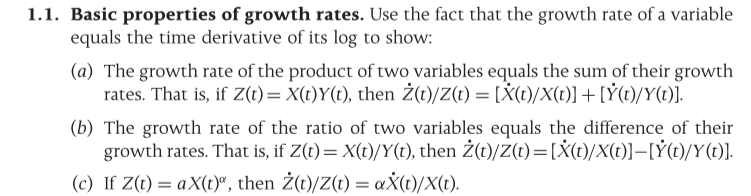
\includegraphics[width=\textwidth]{./HW1-DR1.1.png}
        \end{figure}
        
        We have by the chain rule that
        \begin{align}
            \frac{ d\ln{x(t)} }{ dt } = \frac{ 1 }{ x(t) } \frac{ dx(t) }{ dt } = \frac{ \dot{x}(t) }{ x(t) }
        \end{align}
        
    
    \subsection{Z(t) = X(t)Y(t)}
    
        \begin{align*}
            Z(t) = X(t)Y(t)
            \implies&
            \ln(Z(t)) = \ln(X(t)) + \ln(Y(t))
            \\ \implies&
            \frac{ d \ln(Z(t)) }{ dt }
            = \frac{ d\ln(X(t)) }{ dt } + \frac{ d\ln(Y(t)) }{ dt }
            \\ \implies&
            \frac{ \dot{Z}(t) }{ Z(t) }
            = \frac{ \dot{X}(t) }{ X(t) } + \frac{ \dot{Y}(t) }{ Y(t) }
        \end{align*}
    
    \subsection{Z(t) = X(t)/Y(t)}
        
        \begin{align*}
            Z(t) = \frac{X(t)}{Y(t)}
            \implies&
            \ln(Z(t)) = \ln(X(t)) - \ln(Y(t))
            \\ \implies&
            \frac{ d \ln(Z(t)) }{ dt }
            = \frac{ d\ln(X(t)) }{ dt } - \frac{ d\ln(Y(t)) }{ dt }
            \\ \implies&
            \frac{ \dot{Z}(t) }{ Z(t) }
            = \frac{ \dot{X}(t) }{ X(t) } - \frac{ \dot{Y}(t) }{ Y(t) }
        \end{align*}
        
    
    \subsection{Z(t) = aX(t)$^\alpha$}
        
        \begin{align*}
            Z(t) = a X(t)^{\alpha}
            \implies&
            \ln(Z(t)) = \ln(a) + \alpha\ln(X(t))
            \\ \implies&
            \frac{ d \ln(Z(t)) }{ dt }
            = \frac{ d\ln(a) }{ dt } + \alpha \frac{ d\ln(X(t)) }{ dt }
            \\ \implies&
            \frac{ \dot{Z}(t) }{ Z(t) }
            = \alpha \frac{ \dot{X}(t) }{ X(t) }
        \end{align*}
    
    \section{Math Review: DR 1.2.}
        
        \begin{figure}[h!]
            \centering
            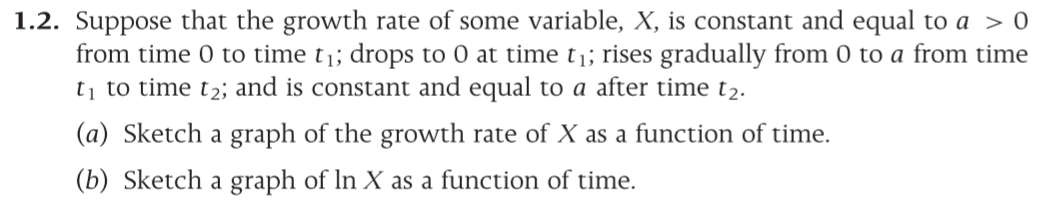
\includegraphics[width=\textwidth]{./HW1-DR1.2.png}
        \end{figure}


        
\end{document}
